\chapter{Calibration of Gorokhovski's breakup model}
\label{app:second_atom_goro_calibration}


The Gorokhovski stochatic model, described in $\S$\ref{subsec:ch4_goro_model}, presents two free constants $K_1$ and $K_2$ in Eq. (\ref{eq:gorokhovski_epsilon_parameters_definition}) which can be tuned for each particular case and which affect the size of the children droplets produced.  $K_1$ affects the mean value of the generated children particles a breakup event, while $K_2$ controls the deviation from this mean \citepColor[senoner_simulation_2010]. The effect of both constants in the sprays have been investigated by selecting a baseline configuration with $K_1 = 0.05$, $K_2 = 1.0$ (such values provided the best experimental comparison obtained in terms of SMD) and varying both constants independently: first $K_1$ is increased to $0.1$ and $0.2$, and then $K_2$ is decreased to 0.5 and 0.25, making a total of five simulations reported. 

Results for global SMD and experimental deviations $\varepsilon_\mathrm{SMD}$, Eq. (\ref{eq:error_expe_SMD_LGS_simus}), are given in Table \ref{tab:SMD_deviations_Gorokhovski}. Maps of SMD and flux are shown in Figure \ref{fig:maps_LGS_JICF_second_atom_apte_calibration}, their integrated profiles in Figure \ref{fig:profiles_LGS_JICF_apte_calibration}, and the evolution of SMD along the channel is represented in Figure \ref{fig:SMD_vs_x_param_goro_calibration}. In general, it can be stated that:

\begin{itemize}

	\item By increasing $K_1$, the global SMD decreases. The spray vertical boundary decreases. Hence, maximum local fluxes retrieved are larger, due to a more concentrated spray.
	
	\item By increasing $K_2$, the global SMD increases. Modifications in $K_2$ lead to bigger differences in the SMD errors as shown in Table \ref{tab:SMD_deviations_Gorokhovski}, which indicates that this constant has a greater influence on the atomization than $K_2$. Also, the spray vertical boundary increases. 

\end{itemize}



From this analysis, the constants $K_1 = 0.05$, $K_2 = 1.0$ were chosen for performing the rest of the analyses from Chapter \ref{ch6:jicf_lgs_simulations} since they yield the lowest error in SMD with respect to experiments. 




\begin{table}[!h]
\centering
\caption{SMD values at $x = 80$ mm obtained with different constants in the Gorokhovski secondary atomization model}
\begin{tabular}{ccc}
\thickhline
Case & $SMD~\left[\mu \mathrm{m} \right]$ & $\varepsilon_{SMD}~\left[\% \right]$ \\
\thickhline
Experiments & 31 & - \\
$K_1 = 0.05,~K_2 = 0.25$ & 16.60 & -46.45 \\
$K_1 = 0.05,~K_2 = 0.5$ & 18.74 & -39.55 \\
$K_1 = 0.05,~K_2 = 1.0$ & 19.52 & -37.03 \\
$K_1 = 0.10,~K_2 = 1.0$ & 18.57 & -40.11 \\
$K_1 = 0.20,~K_2 = 1.0$ & 17.58 & -43.28 \\
\thickhline
\end{tabular}
\label{tab:SMD_deviations_Gorokhovski}
\end{table}



\clearpage


\begin{figure}[t!]
\flushleft
\begin{subfigure}[b]{0.2\textwidth}
	\flushleft
%	\hspace*{-0.35in}
   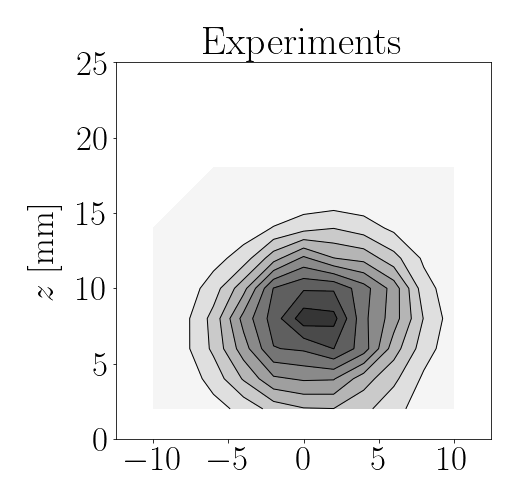
\includegraphics[scale=0.4]{./part2_developments/figures_ch6_lagrangian_JICF/apte_model_calibration_u_vw_lognorm/maps/expe_flux}
   %\label{} 
\end{subfigure}
\hspace*{0.27in}
\begin{subfigure}[b]{0.2\textwidth}
	\flushleft
   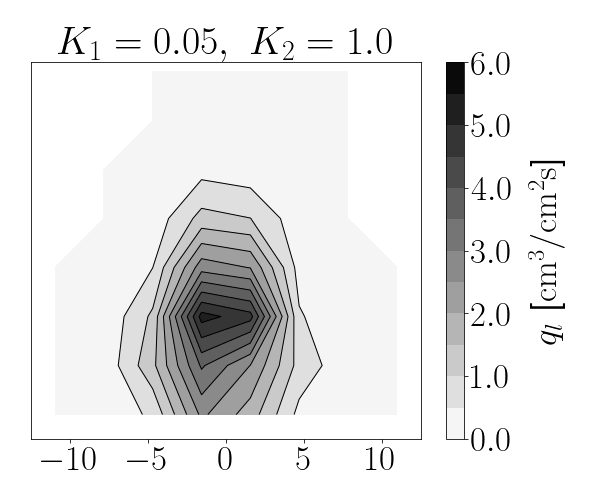
\includegraphics[scale=0.4]{./part2_developments/figures_ch6_lagrangian_JICF/apte_model_calibration_u_vw_lognorm/maps/k1_0p05_k2_1p0_flux}
   %\label{} 
\end{subfigure}
\hspace*{0.02in}
\begin{subfigure}[b]{0.2\textwidth}
	\flushleft
   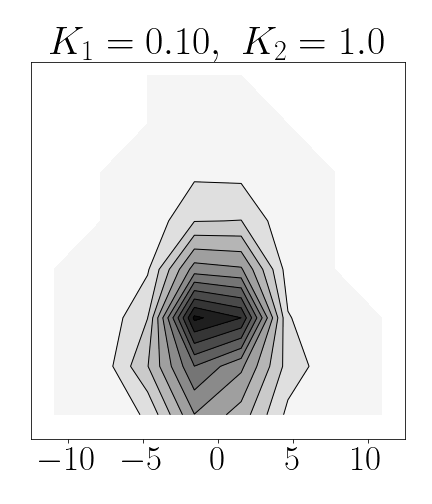
\includegraphics[scale=0.4]{./part2_developments/figures_ch6_lagrangian_JICF/apte_model_calibration_u_vw_lognorm/maps/k1_0p10_k2_1p0_flux}
   %\label{} 
\end{subfigure}
\hspace*{0.02in}
\begin{subfigure}[b]{0.2\textwidth}
	\flushleft
   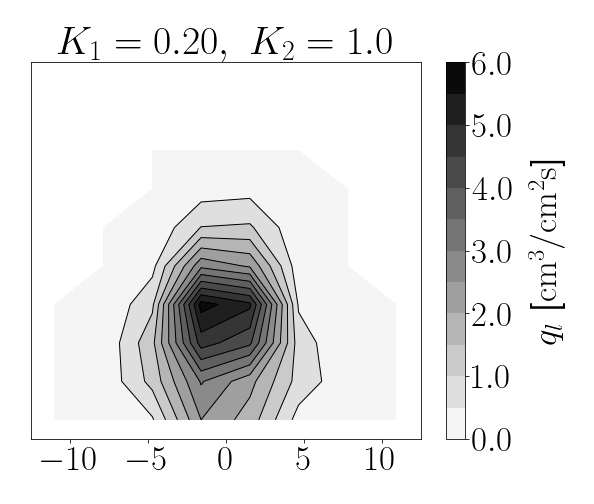
\includegraphics[scale=0.4]{./part2_developments/figures_ch6_lagrangian_JICF/apte_model_calibration_u_vw_lognorm/maps/k1_0p20_k2_1p0_flux}
   %\label{} 
\end{subfigure}

\vspace*{-0.25in}

\flushleft
\begin{subfigure}[b]{0.2\textwidth}
	\flushleft
%	\hspace*{-0.35in}
   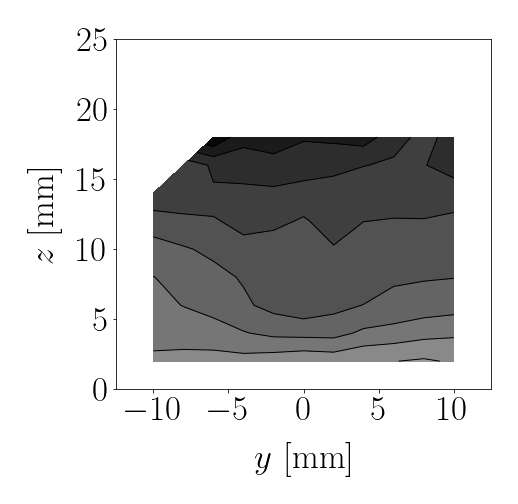
\includegraphics[scale=0.4]{./part2_developments/figures_ch6_lagrangian_JICF/apte_model_calibration_u_vw_lognorm/maps/expe_SMD}
   %\label{} 
\end{subfigure}
\hspace*{0.27in}
\begin{subfigure}[b]{0.2\textwidth}
	\flushleft
   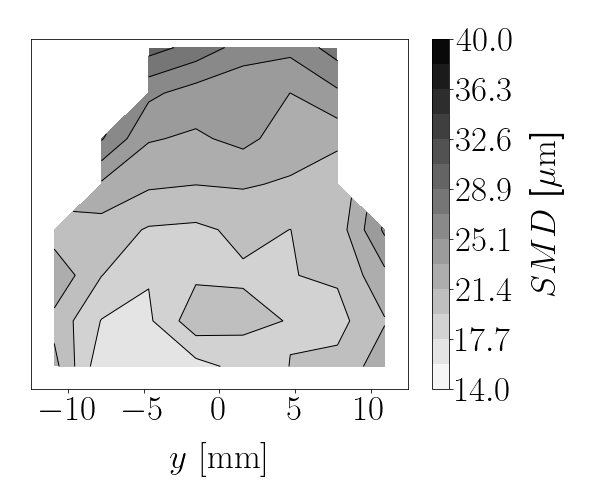
\includegraphics[scale=0.4]{./part2_developments/figures_ch6_lagrangian_JICF/apte_model_calibration_u_vw_lognorm/maps/k1_0p05_k2_1p0_SMD}
   %\label{} 
\end{subfigure}
\hspace*{0.02in}
\begin{subfigure}[b]{0.2\textwidth}
	\flushleft
   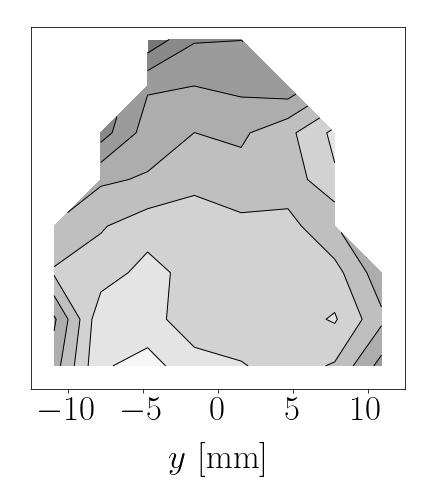
\includegraphics[scale=0.4]{./part2_developments/figures_ch6_lagrangian_JICF/apte_model_calibration_u_vw_lognorm/maps/k1_0p10_k2_1p0_SMD}
   %\label{} 
\end{subfigure}
\hspace*{0.02in}
\begin{subfigure}[b]{0.2\textwidth}
	\flushleft
   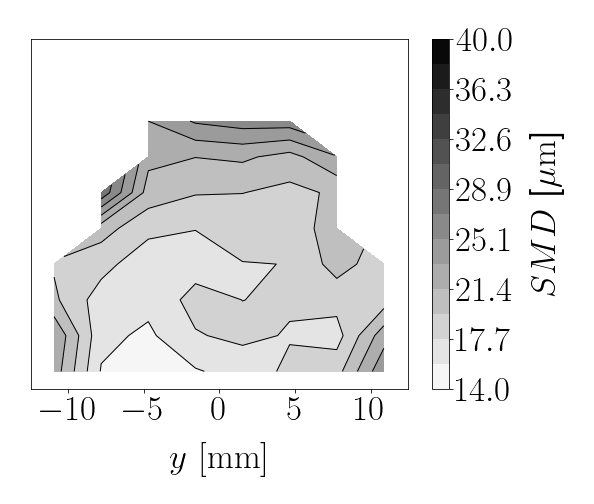
\includegraphics[scale=0.4]{./part2_developments/figures_ch6_lagrangian_JICF/apte_model_calibration_u_vw_lognorm/maps/k1_0p20_k2_1p0_SMD}
   %\label{} 
\end{subfigure}

\vskip\baselineskip
\begin{subfigure}[b]{0.2\textwidth}
	\flushleft
%	\hspace*{-0.35in}
   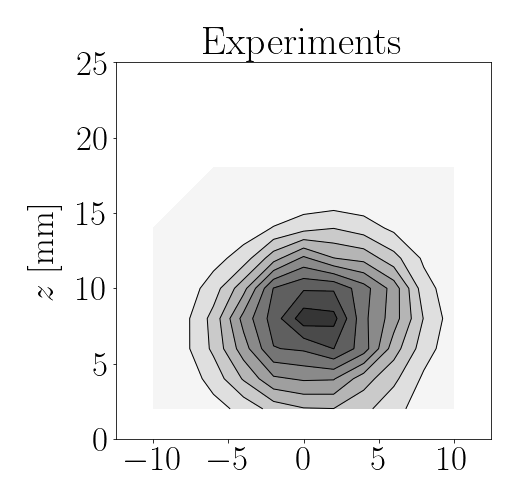
\includegraphics[scale=0.4]{./part2_developments/figures_ch6_lagrangian_JICF/apte_model_calibration_u_vw_lognorm/maps/expe_flux}
   %\label{} 
\end{subfigure}
\hspace*{0.27in}
\begin{subfigure}[b]{0.2\textwidth}
	\flushleft
   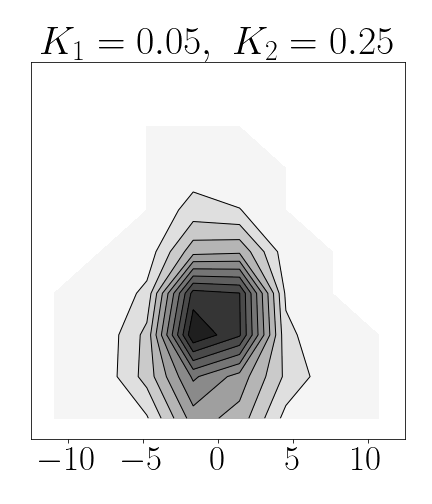
\includegraphics[scale=0.4]{./part2_developments/figures_ch6_lagrangian_JICF/apte_model_calibration_u_vw_lognorm/maps/k1_0p05_k2_0p1_flux}
   %\label{} 
\end{subfigure}
\hspace*{0.02in}
\begin{subfigure}[b]{0.2\textwidth}
	\flushleft
   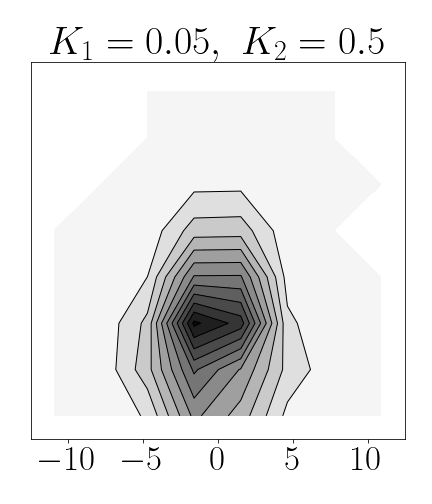
\includegraphics[scale=0.4]{./part2_developments/figures_ch6_lagrangian_JICF/apte_model_calibration_u_vw_lognorm/maps/k1_0p05_k2_0p5_flux}
   %\label{} 
\end{subfigure}
\hspace*{0.02in}
\begin{subfigure}[b]{0.2\textwidth}
	\flushleft
   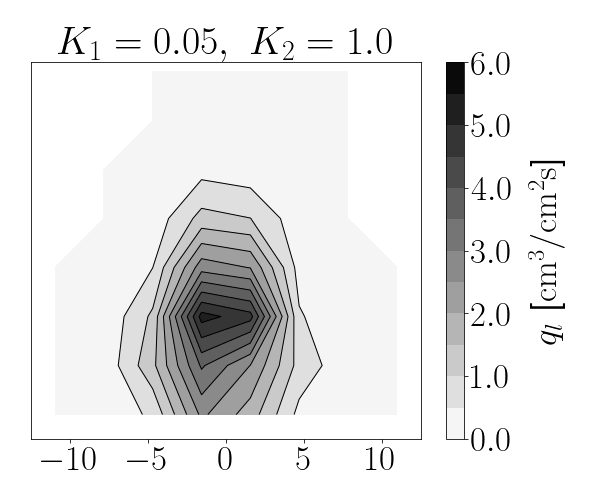
\includegraphics[scale=0.4]{./part2_developments/figures_ch6_lagrangian_JICF/apte_model_calibration_u_vw_lognorm/maps/k1_0p05_k2_1p0_flux}
   %\label{} 
\end{subfigure}

\vspace*{-0.25in}

\flushleft
\begin{subfigure}[b]{0.2\textwidth}
	\flushleft
%	\hspace*{-0.35in}
   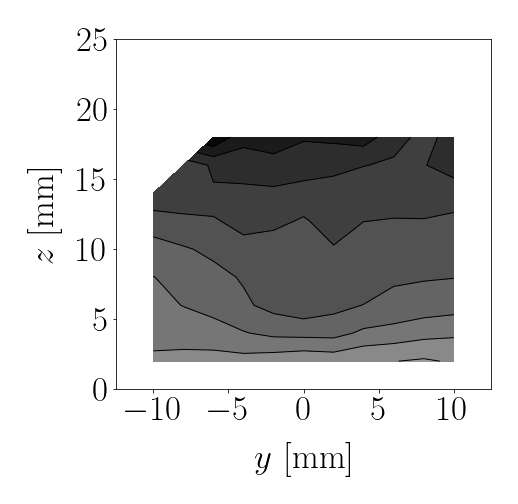
\includegraphics[scale=0.4]{./part2_developments/figures_ch6_lagrangian_JICF/apte_model_calibration_u_vw_lognorm/maps/expe_SMD}
   %\label{} 
\end{subfigure}
\hspace*{0.27in}
\begin{subfigure}[b]{0.2\textwidth}
	\flushleft
   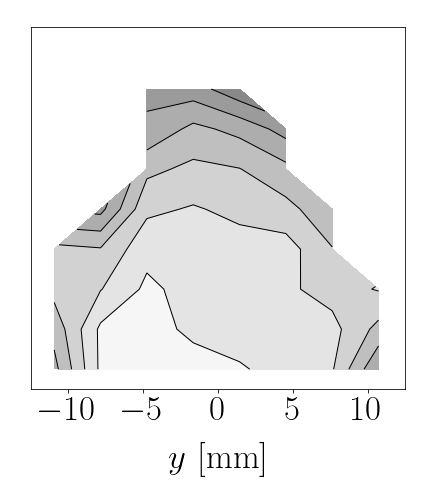
\includegraphics[scale=0.4]{./part2_developments/figures_ch6_lagrangian_JICF/apte_model_calibration_u_vw_lognorm/maps/k1_0p05_k2_0p1_SMD}
   %\label{} 
\end{subfigure}
\hspace*{0.02in}
\begin{subfigure}[b]{0.2\textwidth}
	\flushleft
   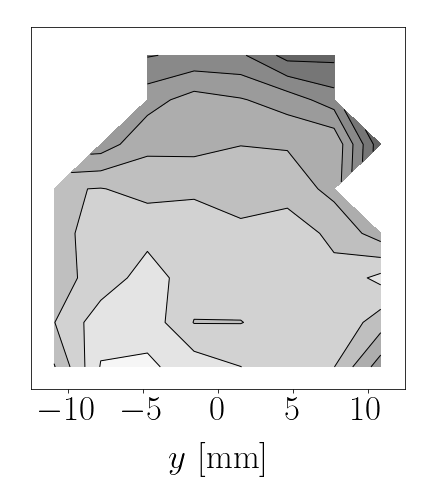
\includegraphics[scale=0.4]{./part2_developments/figures_ch6_lagrangian_JICF/apte_model_calibration_u_vw_lognorm/maps/k1_0p05_k2_0p5_SMD}
   %\label{} 
\end{subfigure}
\hspace*{0.02in}
\begin{subfigure}[b]{0.2\textwidth}
	\flushleft
   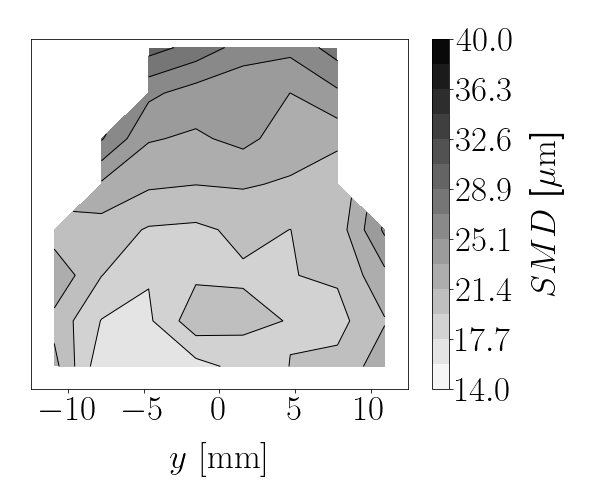
\includegraphics[scale=0.4]{./part2_developments/figures_ch6_lagrangian_JICF/apte_model_calibration_u_vw_lognorm/maps/k1_0p05_k2_1p0_SMD}
   %\label{} 
\end{subfigure}


\caption{Flux and SMD maps for numerical simulations comparing the effect of calibrating the constants from the Gorokhovski model with the experimental results}
\label{fig:maps_LGS_JICF_second_atom_apte_calibration}
\end{figure}


\clearpage


\begin{figure}[t!]
\flushleft
\begin{subfigure}[b]{0.2\textwidth}
	\flushleft
   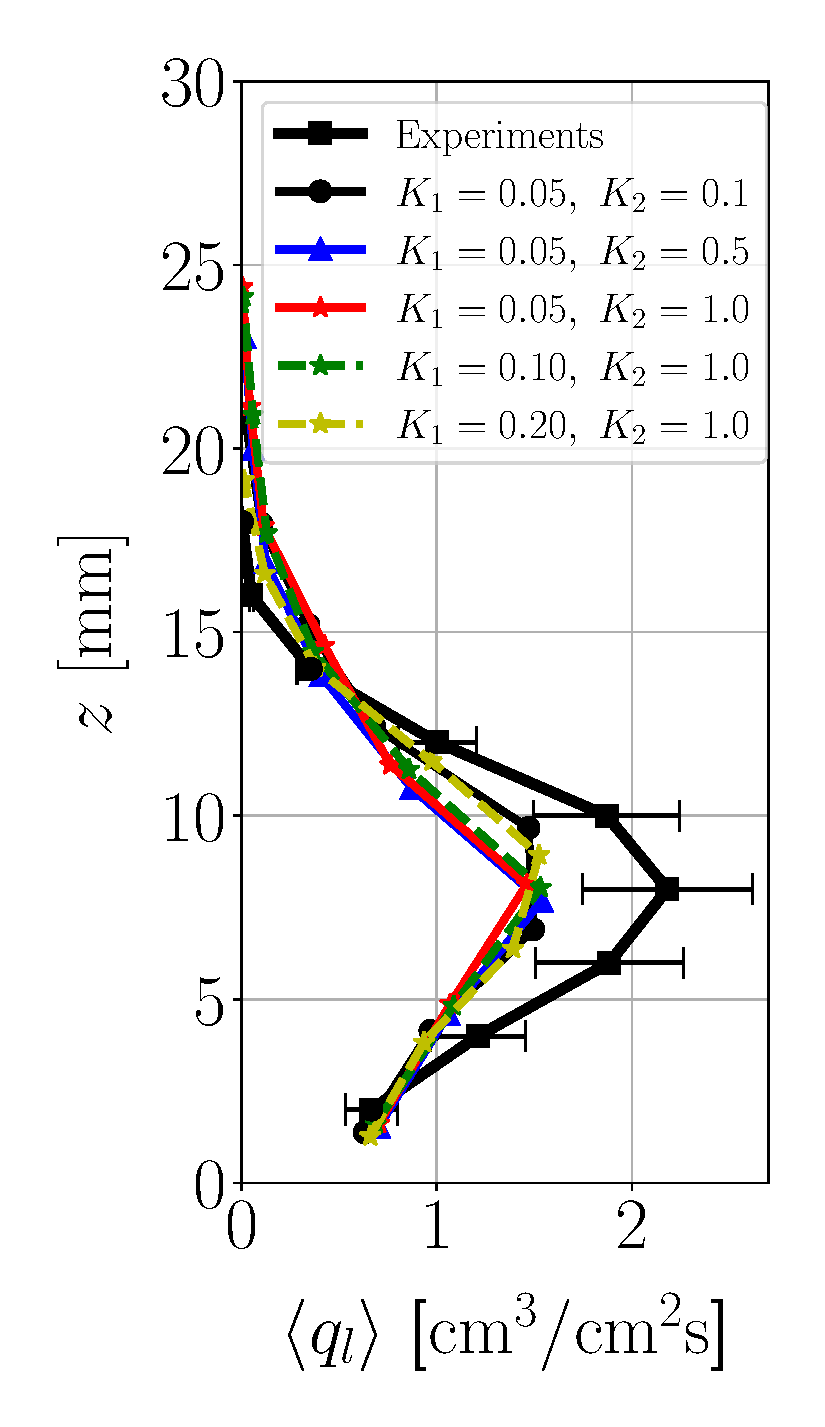
\includegraphics[scale=0.35]{./part2_developments/figures_ch6_lagrangian_JICF/apte_model_calibration_u_vw_lognorm/profiles/flux_along_z}
   %\label{} 
\end{subfigure}
\hspace*{0.5in}
\begin{subfigure}[b]{0.2\textwidth}
	\flushleft
   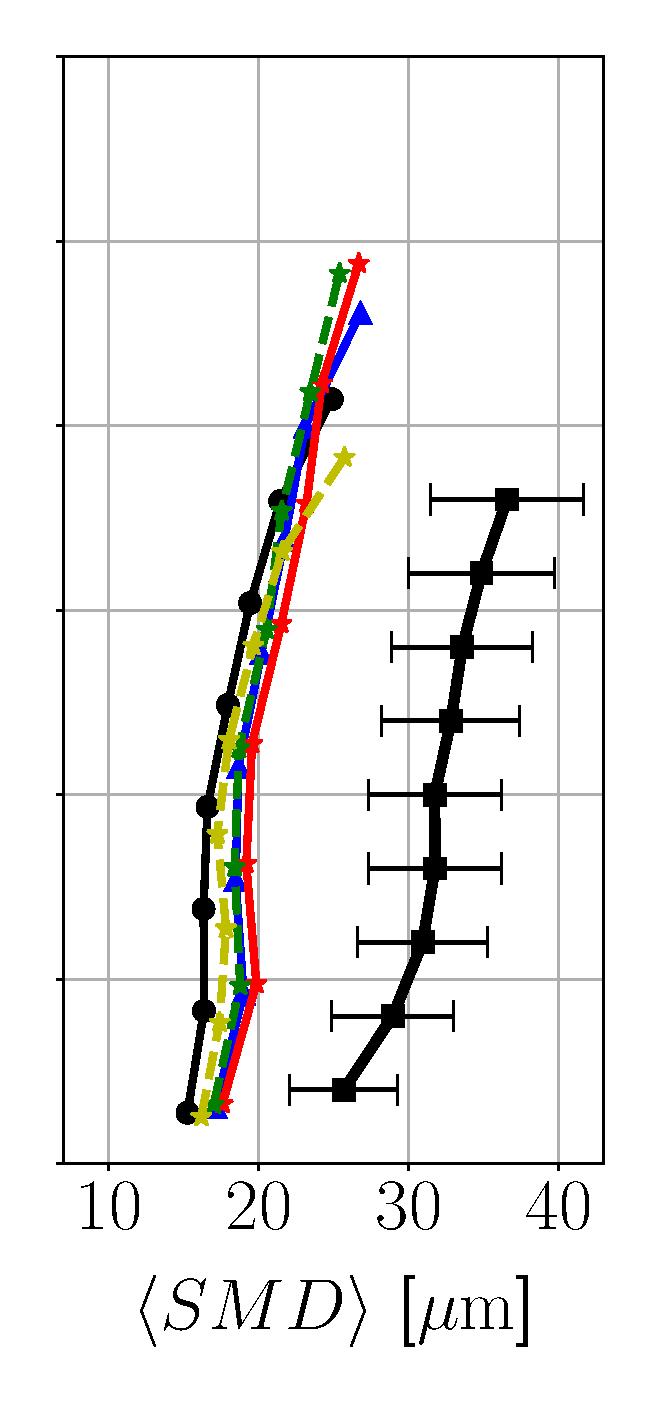
\includegraphics[scale=0.35]{./part2_developments/figures_ch6_lagrangian_JICF/apte_model_calibration_u_vw_lognorm/profiles/SMD_along_z}
   %\label{} 
\end{subfigure}
\hspace*{0.1in}
\begin{subfigure}[b]{0.4\textwidth}
	\flushleft
   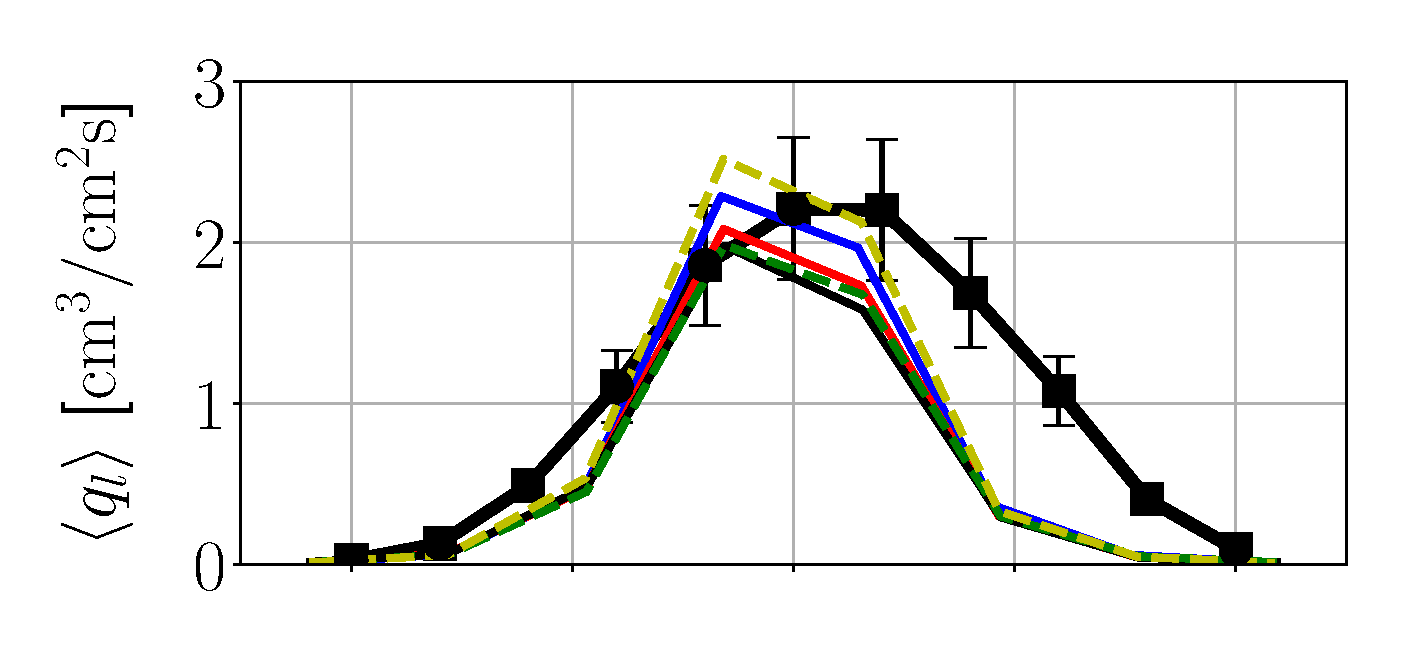
\includegraphics[scale=0.35]{./part2_developments/figures_ch6_lagrangian_JICF/apte_model_calibration_u_vw_lognorm/profiles/flux_along_y}\\
   \vspace{-0.16in}
   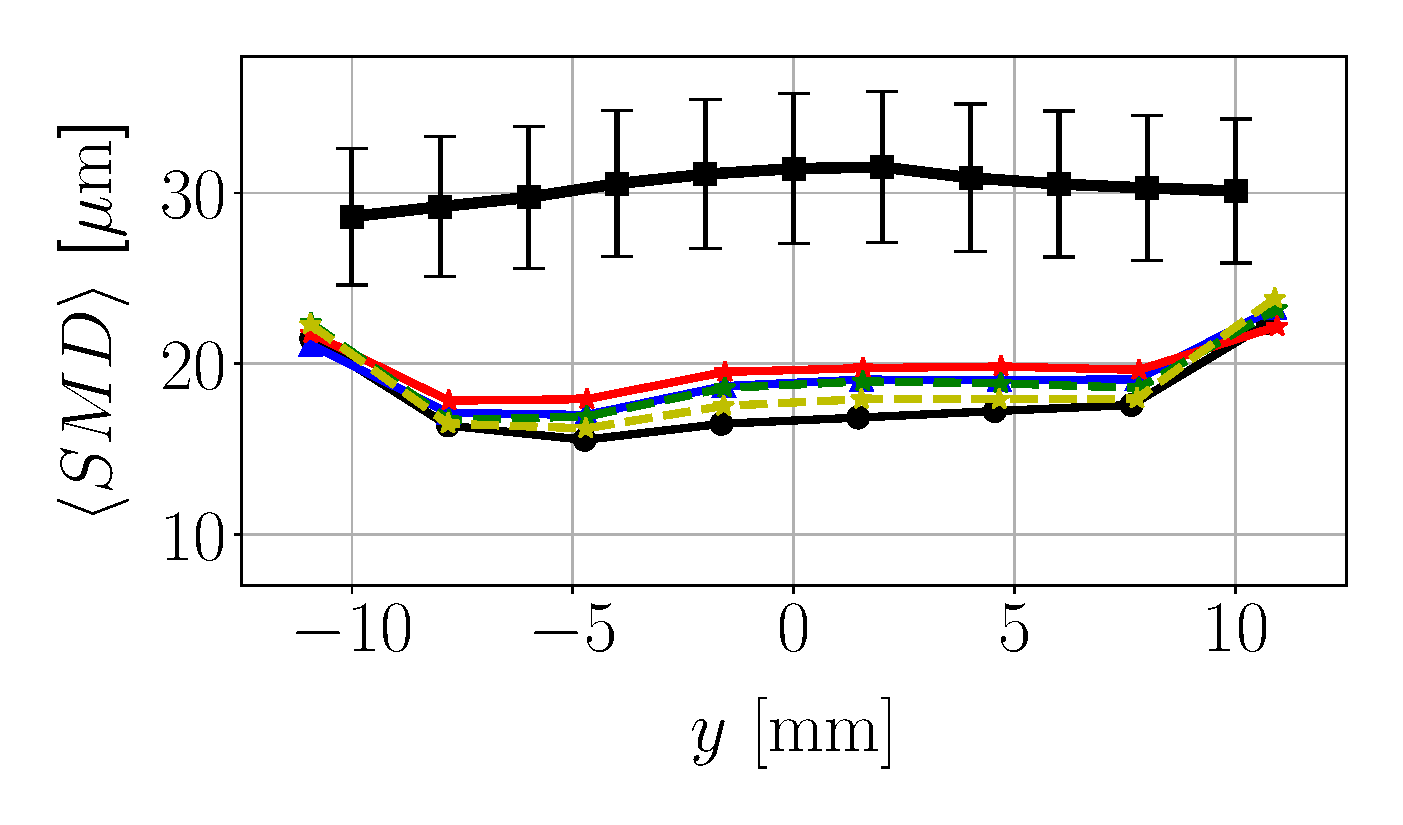
\includegraphics[scale=0.35]{./part2_developments/figures_ch6_lagrangian_JICF/apte_model_calibration_u_vw_lognorm/profiles/SMD_along_y}
   %\label{} 
\end{subfigure}

\caption{Integrated profiles of flux and SMD maps for numerical simulations comparing the effect of Gorokhovski's model calibration with the experimental results}
\label{fig:profiles_LGS_JICF_apte_calibration}
\end{figure}

\begin{figure}[h!]
\centering
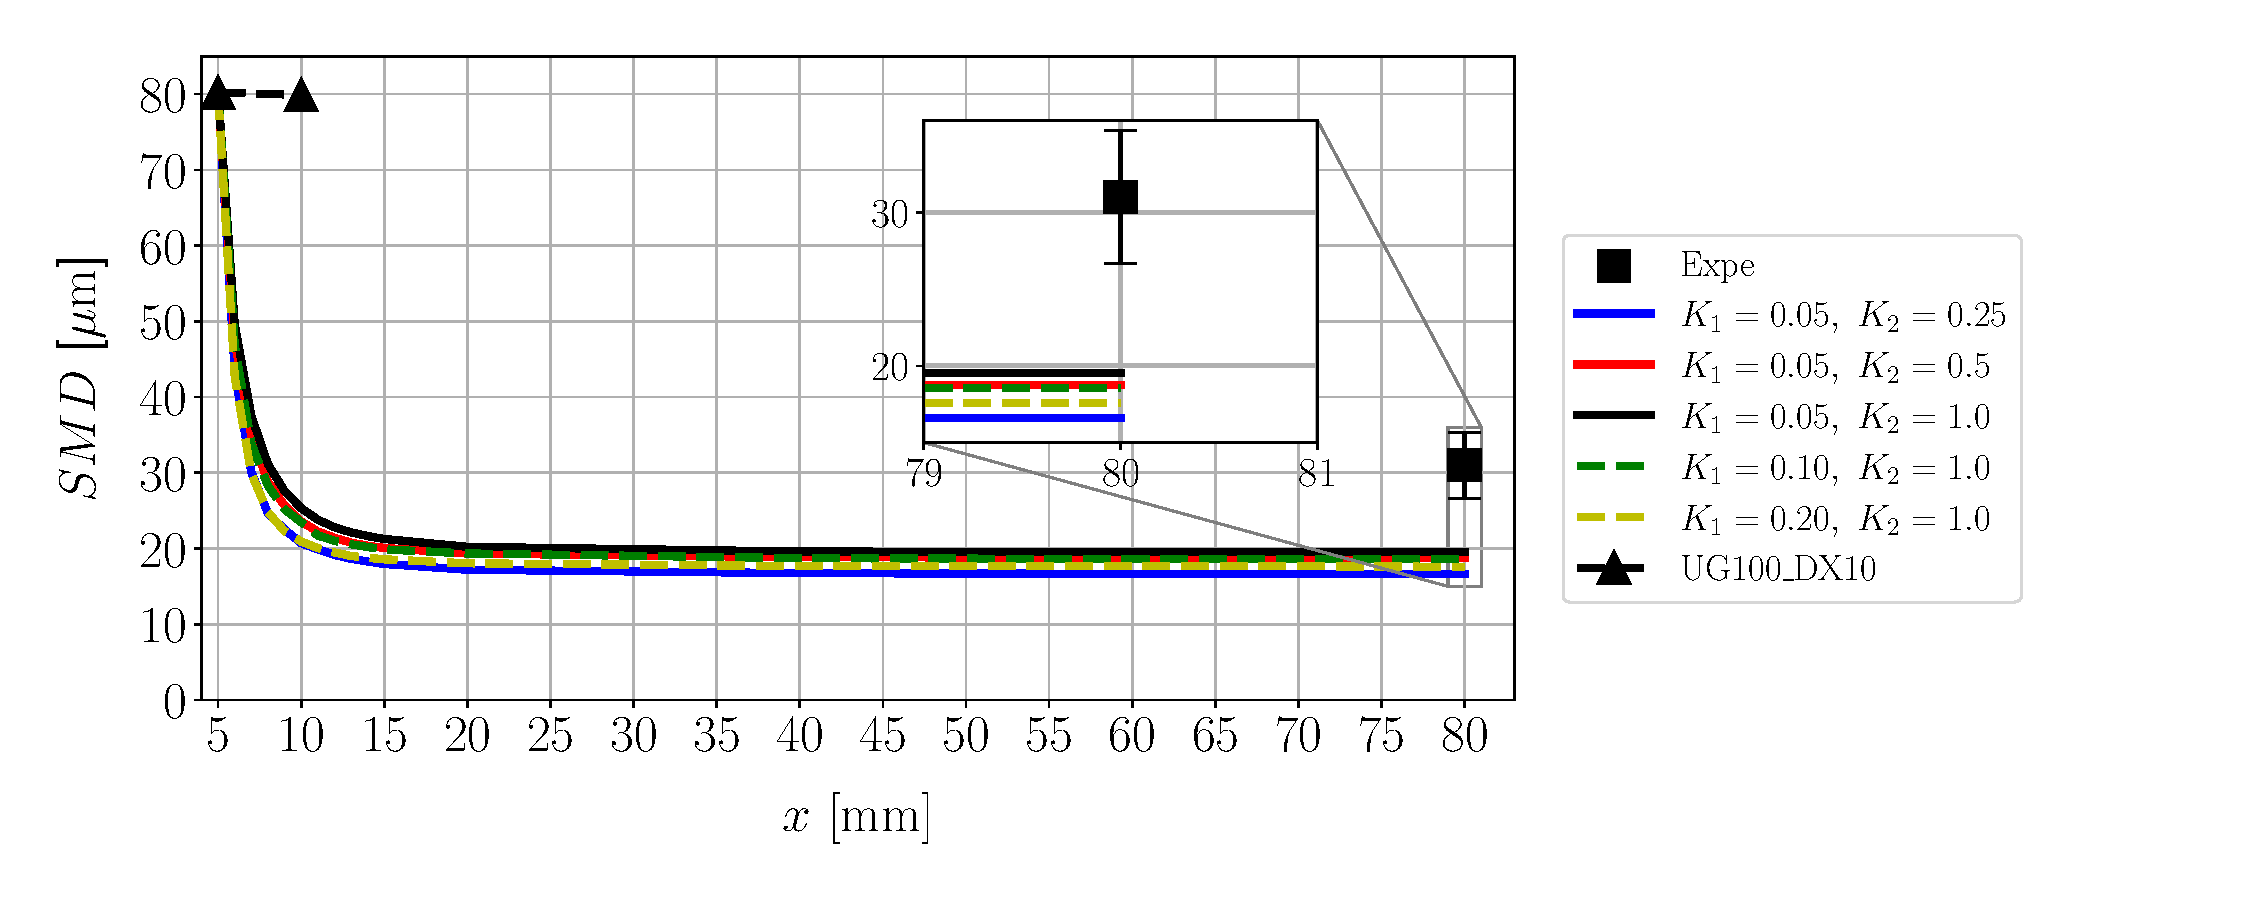
\includegraphics[scale=0.5]{./part2_developments/figures_ch6_lagrangian_JICF/apte_model_calibration_u_vw_lognorm/SMD_vs_x_apte_calibration_comparison}
\caption[Evolution of SMD along axial location $x$ for several values of the Gorokhovski atomization model]{Evolution of SMD along axial location $x$ for several values of constants $K_1$, $K_2$ of the Gorokhovski atomization model. The SMD at $x = 5$ and $10$ mm for the resolved atomization case UG100\_DX10 is also added for comparison}
\label{fig:SMD_vs_x_param_goro_calibration}
\end{figure}





